\documentclass[12pt]{article}
\usepackage[utf8]{inputenc}
\usepackage{lmodern}
\usepackage[T1]{fontenc}
\usepackage{amsmath}
\usepackage{enumitem}
\usepackage{graphicx}
\usepackage{fullpage}
\usepackage{siunitx}
\usepackage{fancyhdr}
\PassOptionsToPackage{hyphens}{url}
\usepackage[hyphens]{url}
\usepackage{color}
\usepackage{enumitem}
\usepackage{textcomp}
\usepackage{geometry}
\usepackage{courier}
\usepackage{listings}
\usepackage{array}
\usepackage{amsthm}
\usepackage{mathdots}
\usepackage{amssymb}
\usepackage{minted}
\usepackage{wrapfig}
\usepackage{titlesec}
\usepackage{parskip}
\usepackage{accents}
\usepackage{gensymb}
\usepackage{indentfirst}
\usepackage{courier}
\usepackage{framed}
\usepackage{etoolbox}
\usepackage{titlesec}
\usepackage{appendix}
\usepackage{mdframed}
\usepackage{verbatim}
\usepackage{xspace}
\usepackage{hyperref}
\AtBeginEnvironment{subappendices}{%
\section*{Appendix}
\addcontentsline{toc}{section}{Appendices}
}



\newcommand{\mytitle}{\textbf{inzva Algorithm Programme 2018-2019\\ \ \\Bundle 13\\ \ \\ Graph-5}}
\title{\vspace{-2em}\mytitle\vspace{-0.3em}}
\author{\textbf{Editor}\\Kayacan Vesek\\ \ \\ \textbf{Reviewer} \\Yasin Kaya}





%\lstset{language=C++,
%                basicstyle=\ttfamily,
%                keywordstyle=\color{blue}\ttfamily,
%                stringstyle=\color{red}\ttfamily,
%                commentstyle=\color{green}\ttfamily,
%                morecomment=[l][\color{magenta}]{\#}
%}

\definecolor{keywordcolor}{rgb}{0,0,0.45}
\definecolor{stringcolor}{rgb}{0.45,0.45,0.45}
\definecolor{commentcolor}{rgb}{0,0.3,0}

\lstset{
language=C++,
basicstyle=\footnotesize\ttfamily,
numbers=left,
%numberstyle=\tiny,
frame=tb,
columns=fullflexible,
showstringspaces=false,
breaklines=true,
tabsize=4,
keywordstyle=\color{keywordcolor}\footnotesize\bf\ttfamily,
stringstyle=\color{stringcolor}\footnotesize\ttfamily,
commentstyle=\color{commentcolor}\it\sffamily
}
% \lstset{basicstyle=\ttfamily,breaklines=true}
\lstloadlanguages{C++}

%\renewcommand{\familydefault}{\sfdefault}

\addtolength{\parskip}{\baselineskip}  
\newcommand{\urlwofont}[1]{\urlstyle{same}\url{#1}}

\renewcommand{\arraystretch}{0.8}
\renewcommand{\headrulewidth}{0pt}
\renewcommand{\footrulewidth}{0pt}

\newcommand{\imagewidth}{0.8\textwidth}

\lhead{}
\chead{}
\rhead{}
\lfoot{}
\cfoot{\thepage}
\rfoot{}

\geometry{
  top=0.9in,
  inner=0.7in,
  outer=0.7in,
  bottom=0.9in,
  headheight=2ex,
  headsep=1ex,
}
\pagestyle{fancy}
%\fancyhf{}
%\setlength{\headsep}{0.2in}


\fancypagestyle{firststyle}
{
    \chead{}
    \setlength{\headsep}{0.0in}
}
\hypersetup{
    unicode=true,
    colorlinks=true,
    linkcolor=blue,
    citecolor=black,
    filecolor=black,
    urlcolor=blue
}

\begingroup
    \makeatletter
    \@for\theoremstyle:=definition,remark,plain\do{%
        \expandafter\g@addto@macro\csname th@\theoremstyle\endcsname{%
            \addtolength\thm@preskip\parskip
            }%
        }
\endgroup

\newtheorem{thm}{Theorem}[section]
\newtheorem{lemma}{Lemma}[section]
\newtheorem{claim}{Claim}[section]
\newtheorem{proposition}{Proposition}[section]
%\theoremstyle{empty}
\newtheorem*{namedthm}{Theorem}


% indention size
%\setlength{\parindent}{19pt}
\setlength{\parindent}{0pt}

% paragraph spacing
\setlength{\parskip}{1em}

% line spacing
\linespread{1}

%\setcounter{tocdepth}{1}

\date{}
\begin{document}

\begin{figure}
  \centering
  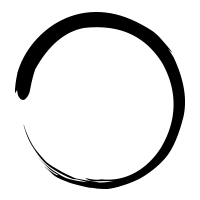
\includegraphics[width=\linewidth/4]{inzva-logo.png}
  \label{fig:inzva}
\end{figure}
\maketitle

\cleardoublepage
\tableofcontents
\markboth{Table of Contents}{}
\cleardoublepage
\newcommand{\sectionbreak}{\clearpage}

%\section{Introduction}
%In this bundle we are going to cover some techniques and algorithms which are used to be solved graph problems (generally trees). 


\section{Eulerian Ordering} 

The Euler tour technique (ETT) is a method in graph theory for representing trees. The tree is viewed as a directed graph that contains two directed edges for each edge in the tree.
\cite{1,2}

\begin{figure}[H]
  \centering
  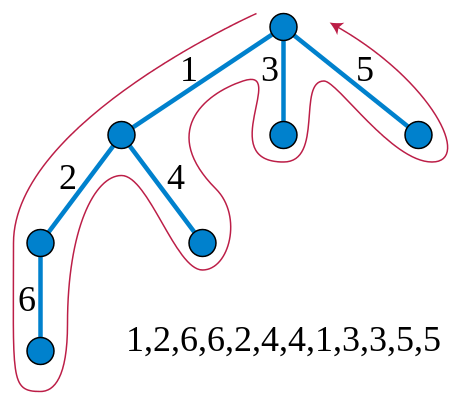
\includegraphics[width=\linewidth/4]{Stirling.png}
  \caption{Euler tour of a tree, with edges labeled to show the order in which they are traversed by the tour \cite{3} }
\end{figure}

\subsection{Construction}

In Euler tour Technique, each vertex is added to the vector twice, while descending via pre-order traversal  into it and while leaving it.
Euler tour tree (ETT) is a method for representing a rooted undirected tree as a number sequence. There are several common ways to build this representation. Usually only the first is called the Euler tour; however, all of them have some pros and cons. 

\begin{figure}[H]
  \centering
  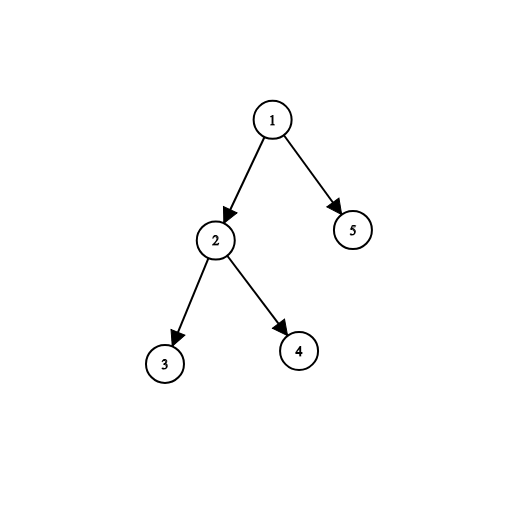
\includegraphics[width=\linewidth/4]{graph3.png}
\end{figure}

The first way is to write down all edges of the tree, directed, in the order of DFS. This is how ETT is defined on \cite{4} . \\ 
$[1-2] [2-3] [3-2] [2-4] [4-2] [2-1] [1-5] [5-1]$\\

The second way is to store vertices. Each vertex is added to the array twice: when we descend into it and when we leave it. Each leaf (except maybe the root) has two consecutive entries.\\
$1 - 2 - 3 - 3 - 4 - 4 - 2 - 5 - 5 - 1$\\
The third way implies storing vertices too, but now each vertex is added every time when we visit it (when descending from the parent and when returning from the child).\\
$1 - 2 - 3 - 2 - 4 - 2 - 1 - 5 - 1$\\

\subsubsection{General Steps to Find ETT}
\begin{itemize}
    \item Start from the root node, initialize discovery time, and assign the root node's discovery time = 1.
    \item Then start a depth first search from the first node, increase the discovery time after every process and assign the node that discovery time.
    \item After visiting all the sub-trees of the node V, assign the discovery time to the finish time of Node V.
\end{itemize}

\begin{minted}[frame=lines,linenos,fontsize=\footnotesize]{c++}
#include <bits/stdc++.h> 
using namespace std; 
vector<int> adj[MAX];  // Adjacency list representation of tree 
// Visited array to keep track visited 
// nodes on tour 
int vis[MAX]; 
// Array to store Euler Tour 
int Euler[2 * MAX]; 
int DiscTime[MAX],FinTime[MAX],time=0;
// Function to add edges to tree 
void add_edge(int u, int v) 
{ 
	adj[u].push_back(v); 
	adj[v].push_back(u); 
} 
// Function to store Euler Tour of tree 
void eulerTree(int u) 
{ 
	vis[u] = 1; 
	Euler[time++] = u; 
	DiscTime[u]=time;
	for (auto it : adj[u]) { 
		if (!vis[it]) { 
			eulerTree(it);
		} 
	} 
	Euler[time++] = u; 
	FinTime[u]=time;
} 
\end{minted}
\section{Segment tree on a Rooted Tree}
As you know, segment tree is for problems with an array. So, obviously we should convert the rooted tree into an array. You know The Euler tour technique, which consists of DFS algorithm and the starting time (the time when we go into a vertex, starting from 1). So, if $S_v$ is the starting time of $v$, element number $S_v$ (in the segment tree) belongs to the vertex number $v$ and if $F_v=max(S_u)+1$ where $u$ is in subtree of $v$, the interval [$S_v$,$F_v$) shows the interval of subtree of $v$ (in the segment tree). \cite{5} 
\subsection{Example : Subtree Sum using Segment Tree}

Lets say there are 2 Queries :

1. Update the value of node $v$ to X.

2. Sum of all the subtrees of node V.


The complexity is $O(QlogN)$.\\
You can use any other data structure that allows to add to the segment and to find a value of an arbitrary element.\\
Also there exists a solution using Heavy-Light decomposition.\\
Source code of update function :
\begin{minted}[frame=lines,linenos,fontsize=\footnotesize]{c++}
void update(int x,int k,int v,int id = 1,int l = 0,int r = n){
	if(s[v] >= r or l >= f[v])	return ;
	if(s[v] <= l && r <= f[v]){ 
	//if we are between start time and the finish time of the Node V
	//All the nodes in this segments(s[v]-f[v]) is in the subtree of node V   
		hkx[id] = (hkx[id] + x) % mod;
		int a = (1LL * h[v] * k) % mod;
		hkx[id] = (hkx[id] + a) % mod;
		sk[id] = (sk[id] + k) % mod;
		return ;
	}
	int mid = (l+r)/2;
	update(x, k, v, 2 * id, l, mid);
	update(x, k, v, 2*id+1, mid, r);
}
\end{minted}
Function for 2nd type query :
\begin{minted}[frame=lines,linenos,fontsize=\footnotesize]{c++}
int ask(int v,int id = 1,int l = 0,int r = n){
	int a = (1LL * h[v] * sk[id]) % mod;
	int ans = (hkx[id] + mod - a) % mod;
	if(r - l < 2)	return ans;
	int mid = (l+r)/2;
	if(s[v] < mid)
		return (ans + ask(v, 2 * id, l, mid)) % mod;
		return (ans + ask(v, 2*id+1, mid, r)) % mod;
}
\end{minted}

\section{Heavy-Light Decomposition} \subsection{Introduction}
In combinatorial mathematics and theoretical computer science, heavy-light decomposition is a technique for decomposing a rooted tree into a set of paths. In a heavy path decomposition, each non-leaf node selects one "heavy edge", the edge to the child that has the greatest number of descendants (breaking ties arbitrarily). The selected edges form the paths of the decomposition.\cite{6} \\
\subsubsection*{Balanced Tree}
So lets think about one tree, if it is a balanced tree, (A balanced binary tree with N nodes has a height of log N). This gives us the following properties:\cite{7} \\
\begin{itemize}
    \item  You need to visit at most log N nodes to reach the root node from any other node
\item You need to visit at most 2 * log N nodes to reach from any node to any other node in the tree
\end{itemize}
$O(logN)$ is not that bad.
\subsubsection*{Chain}
A chain is a set of nodes connected to one after another. It can be viewed as a simple array of nodes. We can do many operations on array of elements with $O( log N )$ complexity using segment tree / BIT or other data structures. \\
Now, we know that Balanced Binary Trees and arrays are good for computation. We can do a lot of operations with $O( log N )$ complexity on both data structures.
\subsubsection*{Unbalanced Tree}
\textbf{Are unbalanced binary trees bad?} In most cases, yes, because balanced binary trees are more compact than unbalanced binary trees and have a smaller maximum distance from the root to the leaf nodes. But it depends on the application, especially how you traverse from the root node to the leaf nodes and what decision is made when choosing whether to go to the left or right subtree. Balancing a binary tree might change its meaning, so balancing is not always possible. In some applications balancing a binary tree may be possible, but balancing is often deferred to some more convenient time rather than enforcing balance at all times. For example, balancing might be done after x modifications or once per time interval, rather than after every modification.\\
So unbalanced trees are not computation friendly. We shall see how we can deal with unbalanced trees. \\
\subsection{The Basic Idea}
We will divide the tree into vertex-disjoint chains (Meaning no two chains have a node in common) in such a way that, to move from any node in the tree to the root node, we will have to change at most log N chains. To put it in other words, the path from any node to the root can be broken into pieces such that the each piece belongs to only one chain. The essence of this tree decomposition is to split the tree into several paths so that we can reach the root vertex from any $V$ by traversing at most $log n$ paths. In addition, none of these paths should intersect with another.\\
It is clear that if we find such a decomposition for any tree, it will allow us to reduce certain single queries of the form “calculate something on the path from $a$ to $b$” to several queries of the type ”calculate something on the segment $[l;r]$ of the $k^{th}$ path”.
\subsection{Construction Method}
We calculate for each vertex $v$ the size of its subtree s(v) (including v).
Next, we consider all the edges leading to the children of a vertex v. We call an edge heavy if it leads to a vertex c such that:\\
$s(c) \ge \frac{s(v)}{2} \iff \text{edge }(v, c)\text{ is heavy}$ \\
All other edges are labeled light.\\
It is obvious that at most one heavy edge can emanate from one vertex downward, because otherwise the vertex $v$ would have at least two children of size $ \geq s(v)/2$, and therefore the size of subtree of $v$ would be too big.

\subsection{Implementation}

Suppose we have a tree  of n nodes, and we have to perform operations on the tree to answer a number of queries, each can be of one of the two types:
\begin{itemize}
    \item change(a, v): Update weight of the $a^{th}$ edge to v.
\item  maxEdge(a, b):  Print the maximum edge weight on the path from node a to node b. 
\end{itemize}
\subsubsection*{Tree Creation}
 Implementation uses adjacency matrix representation of the tree, for the ease of understanding. One can use adjacency list rep with some changes to the source. If edge number $e$ with weight $w$ exists between nodes $u$ and $v$, we shall store $e$ at $tree[u][v]$ and $tree[v][u]$, and the weight $w$ in a separate linear array of edge weights ($n-1$ edges).    
 \subsubsection*{Setting nodes' size, depth and parent}
 Next we do a DFS on the tree to set up arrays that store parent, subtree size and depth of each node. Another important thing we do at the time of DFS is storing the deeper node of every edge we traverse. This will help us at the time of updating the tree.
\subsubsection*{Decompose}
The decompose function assigns for each vertex $v$ the values head[v] and pos[v], which are respectively the head of the heavy path $v$ belongs to and the position of $v$ on the single segment tree that covers all vertices.


\newpage
\subsection{Code}
\begin{minted}[frame=lines,linenos,fontsize=\footnotesize]{c++}

/* C++ program for Heavy-Light Decomposition of a tree */
#include<bits/stdc++.h> 
using namespace std; 

#define N 1024 

int tree[N][N]; // Matrix representing the tree 

/* a tree node structure. Every node has a parent, depth, 
subtree size, chain to which it belongs and a position 
in base array*/
struct treeNode 
{ 
	int par; // Parent of this node 
	int depth; // Depth of this node 
	int size; // Size of subtree rooted with this node 
	int pos_segbase; // Position in segment tree base 
	int chain; 
} node[N]; 

/* every Edge has a weight and two ends. We store deeper end */
struct Edge 
{ 
	int weight; // Weight of Edge 
	int deeper_end; // Deeper end 
} edge[N]; 

/* we construct one segment tree, on base array */
struct segmentTree 
{ 
	int base_array[N], tree[6*N]; 
} s; 

// A function to add Edges to the Tree matrix 
// e is Edge ID, u and $v$ are the two nodes, w is weight 
void addEdge(int e, int u, int v, int w) 
{ 
	/*tree as undirected graph*/
	tree[u-1][v-1] = e-1; 
	tree[v-1][u-1] = e-1; 

	edge[e-1].weight = w; 
} 

// A recursive function for DFS on the tree 
// curr is the current node, prev is the parent of curr, 
// dep is its depth 
void dfs(int curr, int prev, int dep, int n) 
{ 
	/* set parent of current node to predecessor*/
	node[curr].par = prev; 
	node[curr].depth = dep; 
	node[curr].size = 1; 

	/* for node's every child */
	for (int j=0; j<n; j++) 
	{ 
		if (j!=curr && j!=node[curr].par && tree[curr][j]!=-1) 
		{ 
			/* set deeper end of the Edge as this child*/
			edge[tree[curr][j]].deeper_end = j; 

			/* do a DFS on subtree */
			dfs(j, curr, dep+1, n); 

			/* update subtree size */
			node[curr].size+=node[j].size; 
		} 
	} 
} 

// A recursive function that decomposes the Tree into chains 
void hld(int curr_node, int id, int *edge_counted, int *curr_chain, 
		int n, int chain_heads[]) 
{ 
	/* if the current chain has no head, this node is the first node 
	* and also chain head */
	if (chain_heads[*curr_chain]==-1) 
		chain_heads[*curr_chain] = curr_node; 

	/* set chain ID to which the node belongs */
	node[curr_node].chain = *curr_chain; 

	/* set position of node in the array acting as the base to 
	the segment tree */
	node[curr_node].pos_segbase = *edge_counted; 

	/* update array which is the base to the segment tree */
	s.base_array[(*edge_counted)++] = edge[id].weight; 

	/* Find the special child (child with maximum size) */
	int spcl_chld = -1, spcl_edg_id; 
	for (int j=0; j<n; j++) 
	if (j!=curr_node && j!=node[curr_node].par && tree[curr_node][j]!=-1) 
		if (spcl_chld==-1 || node[spcl_chld].size < node[j].size) 
		spcl_chld = j, spcl_edg_id = tree[curr_node][j]; 

	/* if special child found, extend chain */
	if (spcl_chld!=-1) 
	hld(spcl_chld, spcl_edg_id, edge_counted, curr_chain, n, chain_heads); 

	/* for every other (normal) child, do HLD on child subtree as separate 
	chain*/
	for (int j=0; j<n; j++) 
	{ 
	if (j!=curr_node && j!=node[curr_node].par && 
			j!=spcl_chld && tree[curr_node][j]!=-1) 
	{ 
		(*curr_chain)++; 
		hld(j, tree[curr_node][j], edge_counted, curr_chain, n, chain_heads); 
	} 
	} 
} 

// A recursive function that constructs Segment Tree for array[ss..se). 
// si is index of current node in segment tree st 
int construct_ST(int ss, int se, int si) 
{ 
	// If there is one element in array, store it in current node of 
	// segment tree and return 
	if (ss == se-1) 
	{ 
		s.tree[si] = s.base_array[ss]; 
		return s.base_array[ss]; 
	} 

	// If there are more than one elements, then recur for left and 
	// right subtrees and store the minimum of two values in this node 
	int mid = (ss + se)/2; 
	s.tree[si] = max(construct_ST(ss, mid, si*2), 
					construct_ST(mid, se, si*2+1)); 
	return s.tree[si]; 
} 

// A recursive function that updates the Segment Tree 
// x is the node to be updated to value val 
// si is the starting index of the segment tree 
// ss, se mark the corners of the range represented by si 
int update_ST(int ss, int se, int si, int x, int val) 
{ 

	if(ss > x || se <= x); 

	else if(ss == x && ss == se-1)s.tree[si] = val; 

	else
	{ 
		int mid = (ss + se)/2; 
		s.tree[si] = max(update_ST(ss, mid, si*2, x, val), 
						update_ST(mid, se, si*2+1, x, val)); 
	} 

	return s.tree[si]; 
} 

// A function to update Edge e's value to val in segment tree 
void change(int e, int val, int n) 
{ 
	update_ST(0, n, 1, node[edge[e].deeper_end].pos_segbase, val); 

	// following lines of code make no change to our case as we are 
	// changing in ST above 
	// Edge_weights[e] = val; 
	// segtree_Edges_weights[deeper_end_of_edge[e]] = val; 
} 

// A function to get the LCA of nodes u and $v$ 
int LCA(int u, int v, int n) 
{ 
	/* array for storing path from u to root */
	int LCA_aux[n+5]; 

	// Set u is deeper node if it is not 
	if (node[u].depth < node[v].depth) 
	swap(u, v); 

	/* LCA_aux will store path from node u to the root*/
	memset(LCA_aux, -1, sizeof(LCA_aux)); 

	while (u!=-1) 
	{ 
		LCA_aux[u] = 1; 
		u = node[u].par; 
	} 

	/* find first node common in path from $v$ to root and u to 
	root using LCA_aux */
	while (v) 
	{ 
		if (LCA_aux[v]==1)break; 
		v = node[v].par; 
	} 

	return v; 
} 

/* A recursive function to get the minimum value in a given range 
	of array indexes. The following are parameters for this function. 
	st --> Pointer to segment tree 
	index --> Index of current node in the segment tree. Initially 
			0 is passed as root is always at index 0 
	ss & se --> Starting and ending indexes of the segment represented 
				by current node, i.e., st[index] 
	qs & qe --> Starting and ending indexes of query range */
int RMQUtil(int ss, int se, int qs, int qe, int index) 
{ 
	//printf("%d,%d,%d,%d,%d\n", ss, se, qs, qe, index); 

	// If segment of this node is a part of given range, then return 
	// the min of the segment 
	if (qs <= ss && qe >= se-1) 
		return s.tree[index]; 

	// If segment of this node is outside the given range 
	if (se-1 < qs || ss > qe) 
		return -1; 

	// If a part of this segment overlaps with the given range 
	int mid = (ss + se)/2; 
	return max(RMQUtil(ss, mid, qs, qe, 2*index), 
			RMQUtil(mid, se, qs, qe, 2*index+1)); 
} 

// Return minimum of elements in range from index qs (quey start) to 
// qe (query end). It mainly uses RMQUtil() 
int RMQ(int qs, int qe, int n) 
{ 
	// Check for erroneous input values 
	if (qs < 0 || qe > n-1 || qs > qe) 
	{ 
		printf("Invalid Input"); 
		return -1; 
	} 

	return RMQUtil(0, n, qs, qe, 1); 
} 

// A function to move from u to $v$ keeping track of the maximum 
// we move to the surface changing u and chains 
// until u and $v$ donot belong to the same 
int crawl_tree(int u, int v, int n, int chain_heads[]) 
{ 
	int chain_u, chain_v = node[v].chain, ans = 0; 

	while (true) 
	{ 
		chain_u = node[u].chain; 

		/* if the two nodes belong to same chain, 
		* we can query between their positions in the array 
		* acting as base to the segment tree. After the RMQ, 
		* we can break out as we have no where further to go */
		if (chain_u==chain_v) 
		{ 
			if (u==v); //trivial 
			else
			ans = max(RMQ(node[v].pos_segbase+1, node[u].pos_segbase, n), 
						ans); 
			break; 
		} 

		/* else, we query between node u and head of the chain to which 
		u belongs and later change u to parent of head of the chain 
		to which u belongs indicating change of chain */
		else
		{ 
			ans = max(ans, 
					RMQ(node[chain_heads[chain_u]].pos_segbase, 
						node[u].pos_segbase, n)); 

			u = node[chain_heads[chain_u]].par; 
		} 
	} 

	return ans; 
} 

// A function for MAX_EDGE query 
void maxEdge(int u, int v, int n, int chain_heads[]) 
{ 
	int lca = LCA(u, v, n); 
	int ans = max(crawl_tree(u, lca, n, chain_heads), 
				crawl_tree(v, lca, n, chain_heads)); 
	printf("%d\n", ans); 
} 

// driver function 
int main() 
{ 
	/* fill adjacency matrix with -1 to indicate no connections */
	memset(tree, -1, sizeof(tree)); 

	int n = 11; 

	/* arguments in order: Edge ID, node u, node v, weight w*/
	addEdge(1, 1, 2, 13); 
	addEdge(2, 1, 3, 9); 
	addEdge(3, 1, 4, 23); 
	addEdge(4, 2, 5, 4); 
	addEdge(5, 2, 6, 25); 
	addEdge(6, 3, 7, 29); 
	addEdge(7, 6, 8, 5); 
	addEdge(8, 7, 9, 30); 
	addEdge(9, 8, 10, 1); 
	addEdge(10, 8, 11, 6); 

	/* our tree is rooted at node 0 at depth 0 */
	int root = 0, parent_of_root=-1, depth_of_root=0; 

	/* a DFS on the tree to set up: 
	* arrays for parent, depth, subtree size for every node; 
	* deeper end of every Edge */
	dfs(root, parent_of_root, depth_of_root, n); 

	int chain_heads[N]; 

	/*we have initialized no chain heads */
	memset(chain_heads, -1, sizeof(chain_heads)); 

	/* Stores number of edges for construction of segment 
	tree. Initially we haven't traversed any Edges. */
	int edge_counted = 0; 

	/* we start with filling the 0th chain */
	int curr_chain = 0; 

	/* HLD of tree */
	hld(root, n-1, &edge_counted, &curr_chain, n, chain_heads); 

	/* ST of segregated Edges */
	construct_ST(0, edge_counted, 1); 

	/* Since indexes are 0 based, node 11 means index 11-1, 
	8 means 8-1, and so on*/
	int u = 11, $v$ = 9; 
	cout << "Max edge between " << u << " and " << $v$ << " is "; 
	maxEdge(u-1, v-1, n, chain_heads); 

	// Change value of edge number 8 (index 8-1) to 28 
	change(8-1, 28, n); 

	cout << "After Change: max edge between " << u << " and "
		<< $v$ << " is "; 
	maxEdge(u-1, v-1, n, chain_heads); 

	v = 4; 
	cout << "Max edge between " << u << " and " << $v$ << " is "; 
	maxEdge(u-1, v-1, n, chain_heads); 

	// Change value of edge number 5 (index 5-1) to 22 
	change(5-1, 22, n); 
	cout << "After Change: max edge between " << u << " and "
		<< $v$ << " is "; 
	maxEdge(u-1, v-1, n, chain_heads); 

	return 0; 
} 
\end{minted}


\section{Centroid Decomposition of Tree}
\subsection{Finding The Centroid}
\subsubsection{Problem Description}
Let $T$ be an undirected tree. Find a node $v$ such that if we delete $v$ from
the tree, spliting it into a forest, each of the trees in the forest would all
have fewer than half the number of vertices from the original tree.\cite{9}
\subsubsection{Solution}
Let $T$ be an undirected tree with $n$ nodes. Choose any arbitrary node $v$ in the tree. If $v$ satisfies the mathematical definition for the centroid, we have our centroid. If else, we know that our mathematical inequality did not hold, and from this we conclude that there exists some $u$ adjacent to $v$ such that $S(u) > n/2$. We make that u our new $v$ and recurse.\\
We never revisit a node because when we decide to move away from it to a node with subtree size greater than$n/2$, we sort of declare that it now belongs to the component with nodes less than $n/2$, and we shall never find our centroid there.\\
In any case we are moving towards the centroid. Also, there are finitely many vertices in the tree. The process must stop, and it will, at the desired vertex.\cite{9}\\
\subsubsection{Step by Step Algortihm}
\begin{itemize}
    \item Step 1: Select arbitrary node v
    \item Step 2: Start a DFS from v, and setup subtree sizes
    \item Step 3: Re-position to node $v$ (or start at any arbitrary $v$ that belongs to the tree)
    \item Step 4: Check mathematical condition of centroid for v
    \item Step 5: If condition passed, return current node as centroid
    \item Step 6: Else move to adjacent node with ‘greatest’ subtree size, and back to step 4
\end{itemize}
\subsubsection{Time Complexity}
$O(n)$ to compute the size of subtrees, and $O(n)$ to find the correct node,
because the cost of the node search is $$\sum_{v\in V}^{} (1 + deg(v)) = 2n-1$$

Therefore, the time complexity is O(n).

\subsection{Centroid Decomposition}
The solution of the previous problem finds a node $v$ which we shall call a
centroid of the tree. Now what happens if we apply the algorithm
recursively to each subtree split by the centroid?
\begin{itemize}
    \item We get a tree of centroids, which we shall call the centroid
decomposition of the tree.
    \item Runtime is $O(n log n)$ because we will recurse at most $log_2 n$ times
    \item Notice this decomposition has $(log\hspace{0.2cm} n$) depth, so we can essentially do divide and conquer on the tree
\end{itemize}
 Algorithm
\begin{itemize}
    \item  Make the centroid as the root of a new tree (which we will call the ‘centroid tree’)
    \item Recursively decompose the trees in the resulting forest
    \item Make the centroids of these trees as children of the centroid which last split them.
\end{itemize}
The centroid tree has depth O(log n), and can be constructed in O(n log n), as we can find the centroid in O(n).
\begin{figure}[H]
  \centering
  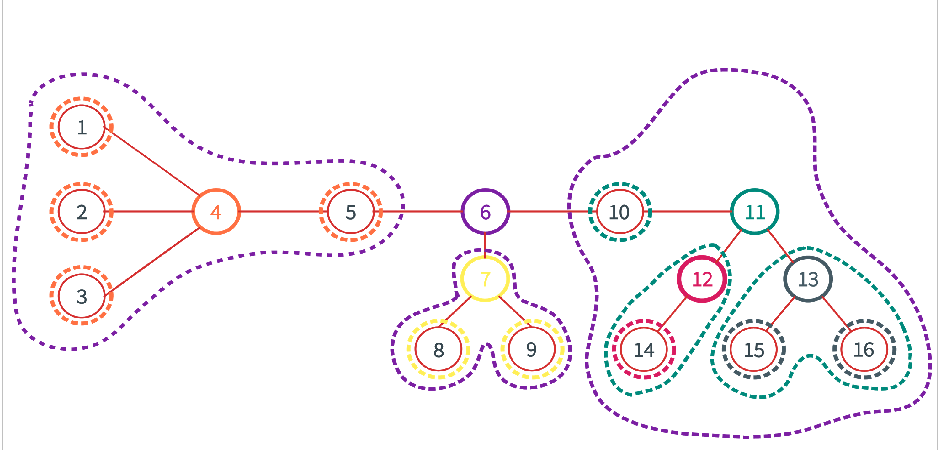
\includegraphics[width=\linewidth]{cd4.png}
  \caption{subtrees generated by a centroid have been surrounded by a dotted line of the same color as the color of centroid. \cite{9} }
\end{figure}
\begin{figure}[H]
  \centering
  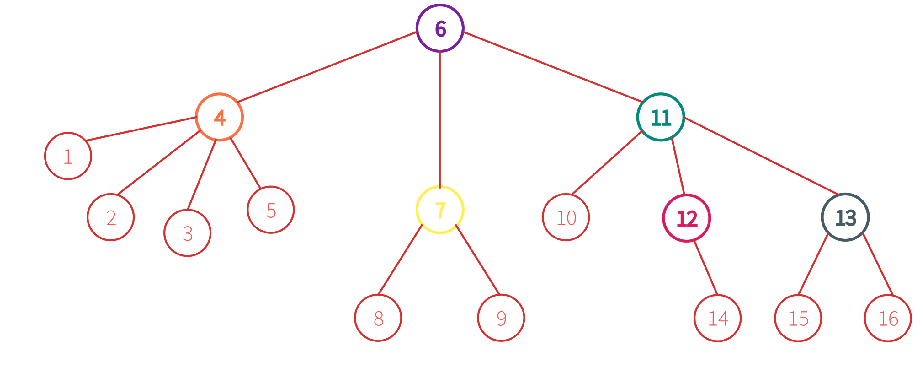
\includegraphics[width=\linewidth]{cd5.png}
  \caption{Final representation of a centroid tree.\cite{9} }
\end{figure}
    
\subsection{Sample Problem and Code}

\subsubsection*{Task Summary}
We’re given an edge weighted tree with N nodes and an integer K. The problem asks us to compute the path with the fewest edges such that the sum of the weights of the edges is exactly K.\cite{10} \\

\begin{minted}[frame=lines,linenos,fontsize=\footnotesize]{c++}

#include <stdio.h>
#include <stdlib.h>
#include <string.h>
#include <vector>
#include <algorithm>

using namespace std;

typedef pair<int, int> pii;

#define MAXN 200050
#define MAXK 1000050

#define F first
#define S second

int N, K, global_answer; // Input and result variables
int split_node, current_max; // Variables to calculate centroid
int book_keeping; // Book keeping helper

int H[MAXN][2]; // Input variables
int L[MAXN];

int processed[MAXN]; // Markers to help main recursion
int size[MAXN]; // Size of subtrees in rooted tree
int achievable[MAXK]; // Helper arrays for minimum paths crossing v
int minimum_paths[MAXK];

vector<pii> neighbors[MAXN]; // The actual tree

///////////////////////////////////////////////
//
// Goal: Calculate the size of each subtree
//
///////////////////////////////////////////////
void calc_size(int current, int parent)
{
  size[current] = 0;

  // Recurse on unprocessed nodes and update size
  int i;
  for (i = 0; i < (int)neighbors[current].size(); i++)
    if (!processed[neighbors[current][i].F] && neighbors[current][i].F != parent)
    {
      calc_size(neighbors[current][i].F, current);
      size[current] += 1 + size[neighbors[current][i].F];
    }
}

///////////////////////////////////////////////
//
// Goal: Calculate the centroid
//
///////////////////////////////////////////////
void select_split_node(int current, int parent, int total)
{
  int node_max = (total - size[current] - 1);

  // Recurse on unprocessed nodes updating the maximum subtree on node_max
  int i;
  for (i = 0; i < (int)neighbors[current].size(); i++)
    if (!processed[neighbors[current][i].F] && neighbors[current][i].F != parent)
    {
      select_split_node(neighbors[current][i].F, current, total);
      node_max = max(node_max, 1 + size[neighbors[current][i].F]);
    }

  if (node_max < current_max)
  {
    split_node = current;
    current_max = node_max;
  }
}

///////////////////////////////////////////////
//
// Goal: DFS from the centroid to calculate all paths
//
///////////////////////////////////////////////
void dfs_from_node(int current, int parent, int current_cost, int current_length, int fill)
{
  if (current_cost > K)
    return;

  if (!fill) // If we are calculating the paths
  {
    if (achievable[K - current_cost] == book_keeping)
      if (current_length + minimum_paths[K - current_cost] < global_answer || global_answer == -1)
        global_answer = current_length + minimum_paths[K - current_cost];

    if (current_cost == K)
      if (current_length < global_answer || global_answer == -1)
        global_answer = current_length;
  }
  else // If we are filling the helper array
  {
    if (achievable[current_cost] < book_keeping)
    {
      achievable[current_cost] = book_keeping;
      minimum_paths[current_cost] = current_length;
    }
    else if (current_length < minimum_paths[current_cost])
    {
      achievable[current_cost] = book_keeping;
      minimum_paths[current_cost] = current_length;
    }
  }

  // Recurse on unprocessed nodes
  int i;
  for (i = 0; i < (int)neighbors[current].size(); i++)
    if (!processed[neighbors[current][i].F] && neighbors[current][i].F != parent)
      dfs_from_node(neighbors[current][i].F, current, current_cost + neighbors[current][i].S, current_length + 1, fill);
}

///////////////////////////////////////////////
//
// Goal: Calculate best for subtree
//
///////////////////////////////////////////////
void process(int current)
{
  // Fill the size array
  calc_size(current, -1);

  // Base case
  if (size[current] <= 1)
    return;

  // Calculate the centroid and put it in split_node
  split_node = -1;
  current_max = size[current] + 3;
  select_split_node(current, -1, size[current] + 1);

  // Double dfs to calculate minimums and fill helper array
  book_keeping++;
  int i;
  for (i = 0; i < (int)neighbors[split_node].size(); i++)
    if (!processed[neighbors[split_node][i].F])
    {
      dfs_from_node(neighbors[split_node][i].F, split_node, neighbors[split_node][i].S, 1, 0);
      dfs_from_node(neighbors[split_node][i].F, split_node, neighbors[split_node][i].S, 1, 1);
    }


  int local_split_node = split_node; // Since split_node is global
  processed[split_node] = 1; // Mark as processed to cap recursion

  // Call main method on each subtree from centroid
  for (i = 0; i < (int)neighbors[local_split_node].size(); i++)
    if (!processed[neighbors[local_split_node][i].F])
      process(neighbors[local_split_node][i].F);
}

///////////////////////////////////////////////
//
// Goal: Answer the task
//
///////////////////////////////////////////////
int best_path(int _N, int _K, int H[][2], int L[])
{
  // Reset arrays and variables
  memset(processed, 0, sizeof processed);
  memset(achievable, 0, sizeof achievable);
  memset(minimum_paths, 0, sizeof minimum_paths);
  N = _N;
  K = _K;
  book_keeping = 0;

  // Build tree
  int i;
  for (i = 0; i < N - 1; i++)
  {
    neighbors[H[i][0]].push_back(pii(H[i][1], L[i]));
    neighbors[H[i][1]].push_back(pii(H[i][0], L[i]));
  }

  global_answer = -1;

  // Call main method for whole tree
  process(0);

  return global_answer;
}

///////////////////////////////////////////////
//
// Goal: Read the input
//
///////////////////////////////////////////////
void read_input()
{
  scanf("%d %d", &N, &K);

  int i;
  for (i = 0; i < N - 1; i++)
    scanf("%d %d %d", &H[i][0], &H[i][1], &L[i]);
}

///////////////////////////////////////////////
//
// Goal: Main
//
///////////////////////////////////////////////
int main()
{
  int ans;

  read_input();
  ans = best_path(N, K, H, L);

  printf("%d\n", ans);

  return 0;
}
\end{minted}

\section{Subtrees' Set-Swap Technique (Dsu on Tree)}

Maintain a set of values for each node in the tree. Let set(u) be the set of all values in the subtree rooted at u. We want size(set(u)) for all u.\\
Let a node u have k children, $v_1,v_2...v_k$. Every time you want to merge set(u) with set(vi), pop out the elements from the smaller set and insert them into the larger one. You can think of it like implementing union find, based on size.\\
Consider any arbitrary node value. Every time you remove it from a certain set and insert it into another, the size of the merged set is at least twice the size of the original.\\
Say you merge sets x and y. Assume $size(x)\leq size(y)$. Therefore, by the algorithm, you will push all the elements of x into y. Let xy be the merged set. $size(xy) = size(x)+size(y)$. But  $size(x)\leq size(y)$:\\
So $2*size(x) \leq size(xy) $\\
Thus, each value will not move more than log n times. Since each move is done in $O(logn)$, the total complexity for n values amounts to $O(nlog^2 n)$. \cite{11} \\

\subsection{Implementation}
\subsubsection*{Problem}
Given a tree, every vertex has color. Query is how many vertices in subtree of vertex v are colored with color $c$?
\subsubsection*{Naive Approch}
First, we have to calculate the size of the subtree of every vertices. It can be done with simple dfs:
\begin{minted}[frame=lines,linenos,fontsize=\footnotesize]{c++}
int sz[maxn];
void getsz(int v, int p){
    sz[v] = 1;  // every vertex has itself in its subtree
    for(auto u : g[v])
        if(u != p){
            getsz(u, v);
            sz[v] += sz[u]; // add size of child u to its parent(v)
        }
}
\end{minted}
The $O(N^2)$ Complexity solution as follows:
\begin{minted}[frame=lines,linenos,fontsize=\footnotesize]{c++}
int cnt[maxn];
void add(int v, int p, int x){
    cnt[ col[v] ] += x;
    for(auto u: g[v])
        if(u != p)
            add(u, v, x)
}
void dfs(int v, int p){
    add(v, p, 1);
    //now cnt[c] is the number of vertices in subtree of vertex v that has color c. You can answer the queries easily.
    add(v, p, -1);
    for(auto u : g[v])
        if(u != p)
            dfs(u, v);
}
\end{minted}
\subsubsection{The Set Swap Technique Solution}


\begin{minted}[frame=lines,linenos,fontsize=\footnotesize]{c++}
map<int, int> *cnt[maxn];
void dfs(int v, int p){
    int mx = -1, bigChild = -1;
    for(auto u : g[v])
       if(u != p){
           dfs(u, v);
           if(sz[u] > mx)
               mx = sz[u], bigChild = u;
       }
    if(bigChild != -1)
        cnt[v] = cnt[bigChild];
    else
        cnt[v] = new map<int, int> ();
    (*cnt[v])[ col[v] ] ++;
    for(auto u : g[v])
       if(u != p && u != bigChild){
           for(auto x : *cnt[u])
               (*cnt[v])[x.first] += x.second;
       }
    //now (*cnt[v])[c] is the number of vertices in subtree of vertex v that has color c. You can answer the queries easily.

}
\end{minted}

\begin{thebibliography}{9}

\bibitem{1}
https://www.geeksforgeeks.org/euler-tour-subtree-sum-using-segment-tree/
\bibitem{2}
https://en.wikipedia.org/wiki/Euler\_tour\_technique
\bibitem{3}
https://commons.wikimedia.org/wiki/File:Stirling\_permutation\_Euler\_tour.svg
\bibitem{4}
https://codeforces.com/blog/entry/18369
\bibitem{5}
https://codeforces.com/blog/entry/15890
\bibitem{6}
https://cp-algorithms.com/graph/hld.html
\bibitem{7}
https://blog.anudeep2011.com/heavy-light-decomposition/
\bibitem{8}
https://www.ugrad.cs.ubc.ca/~cs490/2014W2/pdf/jason.pdf
\bibitem{9}
https://www.geeksforgeeks.org/centroid-decomposition-of-tree/
\bibitem{10}
https://github.com/gangsterveggies/IOI-Solutions/blob/master/IOI-2011/race.cpp\bibitem{11}
https://codeforces.com/blog/entry/44351

\end{thebibliography}        

\end{document}
 